
\documentclass[11pt]{article}

%\setlength\topmargin{-0.1in}
%\setlength\headheight{0in}
%\setlength\headsep{0in}
\setlength\textheight{8.5in}
\setlength\textwidth{6.5in}
\setlength\oddsidemargin{0in}
\setlength\evensidemargin{0in}
\setlength{\parindent}{0pt}
\usepackage{placeins}
%\usepackage{indentfirst}
\usepackage{gensymb}
\usepackage{amsmath}
\usepackage{graphicx}
\usepackage{listings}
\usepackage{rotating}
\usepackage{subcaption} 
\usepackage{booktabs}
\usepackage{tikz}
\usepackage{fancyhdr}
\usepackage{pdfpages}
\usepackage{hyperref}
\usepackage{longtable}
\usepackage[toc,page]{appendix}
%For The 2x2 Figure
\usepackage{subcaption}
% To import matlab code
\usepackage{listings}
\usepackage{matlab-prettifier}
\usepackage[framed,numbered,autolinebreaks,useliterate]{mcode}
%Glossary
\usepackage[acronym,nonumberlist]{glossaries}
%\glsaddall %includes all acronymns
%Tables
\usepackage{booktabs}
\newcommand{\ra}[1]{\renewcommand{\arraystretch}{#1}}
%Nomenclature
\usepackage{nomencl}
\makenomenclature
\newif\iffirstglossary\firstglossarytrue
%% This removes the main title:
\renewcommand{\nomname}{}
%% this modifies item separation:
\setlength{\nomitemsep}{15pt}
%% this part defines the groups:
%----------------------------------------------
\usepackage{etoolbox}
\renewcommand\nomgroup[1]{%
  \item[\Large\bfseries
  \ifstrequal{#1}{N}{Nomenclature}{%
  \ifstrequal{#1}{A}{List of Abbreviations}{}}%
]\vspace{10pt}} % this is to add vertical space between the groups.
%----------------------------------------------



\pagestyle{fancy}
\usetikzlibrary{shapes,arrows}
\graphicspath{{Figures/}}
\newcommand{\tabitem}{~~\llap{\textbullet}~~}

\newcommand*{\MyIndent}{\hspace*{0.5cm}}%inerts tab in tables



 
\begin{document} 
\pagenumbering{gobble}

	\begin{titlepage}
	\thispagestyle{empty}
		\newcommand{\HRule}{\rule{\linewidth}{0.5mm}}	
		\center
		\LARGE 
		University of Bath\\
	 	Faculty of Engineering \& Design\\[1cm]	
		%textbf{\Large ME30313 Group Business & Design}\\
		\large
		Word count: 2047\\[0.5cm]
		{\large\today}\\[1cm]	
		\HRule\\[0.4cm]	
		{\LARGE \bfseries Advanced Helicopter Dynamics}\\[0.3cm] 	
		\HRule\\[1cm]	
		\begin{minipage}{0.4\textwidth}
			\begin{flushleft}
				\large
				\textit{Supervisor}\\
				D. \textsc{Cleaver}
			\end{flushleft}
		\end{minipage}
		~
		\begin{minipage}{0.4\textwidth}
			\begin{flushright}
				\large
				\textit{Assessor}\\
				
			\end{flushright}
		\end{minipage}\\[1.4cm]
		\large
		\textit{Author's Candidate Number}\\
		10838\\
		\vfill
		
\includegraphics[width=0.4\textwidth]{UOB_Logo.png}\\
		\vfill 
	\end{titlepage}

%%% ACRONYMS %%

%%END OF ACRONYMS %%%


\thispagestyle{empty}


\section*{Summary}

A computational model was created for the first stage design of a technically optimal blade for a wind turbine using a NACA 0012 aerofoil. The turbine radius was set at 20m with a mean chord of 1m. The optimal design was found by adjusting the linear chord gradient, $c_g$, angular twist rate, $\theta_{TW}$, and initial inclination, $\theta_0$. The initial model was very limited and so tip losses and bending criteria were added, reducing the optimal annual energy production from 59.8\% of the theoretical maximum to 49.7\%. Tip deflection was a limiting factor for the design with optimal designs having the maximum normal tip deflection of 3m. The final optimal values were $c_g = .008 $, $\theta_{TW} = -0.54 \degree /m$ and $\theta_0 = 9.87 \degree$.




\tableofcontents
\thispagestyle{empty}
\listoffigures
\listoftables

\nomenclature[A]{BEMT}{Blade Element Momentum Theory}


%\printnomenclature



\pagenumbering{arabic}
%\setcounter{page}{1}4


\clearpage
%\\\\\\\\\\\\\\\\\\\\\\\\\\\\\\\\\\\\\\\\\\\\\\\\\\\    INTRODUCTION     \\\\\\\\\\\\\\\\\\\\\\\\\\\\\\\\\\\\\\\\\\\\\\\\\\\\\\\\\\\\\\
\section{Introduction}

Over the period 2010 to 2017 total electricity generation in the United Kingdom fell by \mbox{18\% \cite{data1}} as consumption also fell 10\% across the period \cite{data2}. This is in spite of a rising population and number of households. This has been attributed to warmer winters lowering electric heating demands as well as improvements in refrigerator technology and increased use of LED lights \cite{guardian}. Using data made available by the UK Department for Business, Energy \& Industrial Strategy \cite{data1} it can be seen that wind power has defied the slowdown of electricity generation in the UK, rising on average 29\% year on year over the same 2010 to 2017 period as shown by Figure \ref{fig:windgrowth}.

\begin{figure}[ht] 
        \centering
        \begin{subfigure}[b]{0.475\textwidth}
            \centering
            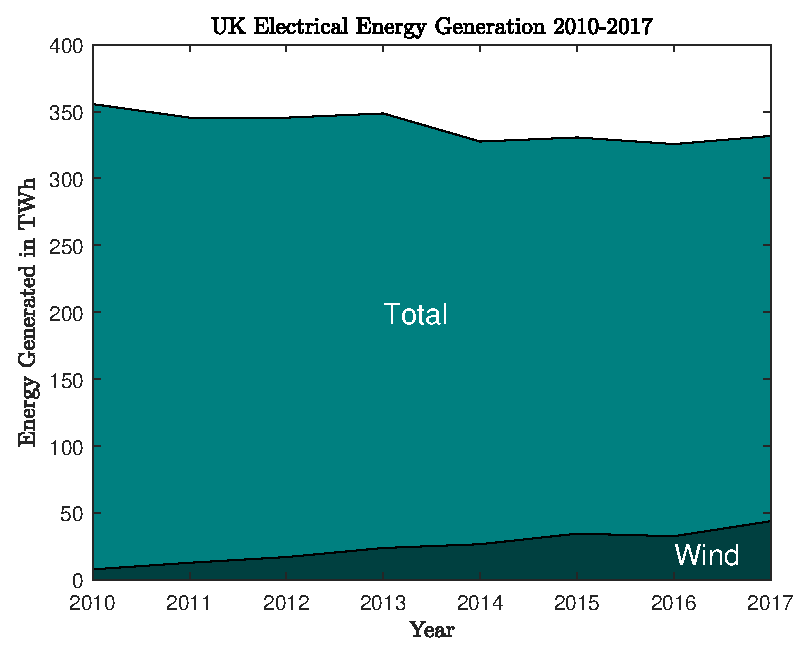
\includegraphics[width=\textwidth]{ukGen}
            \caption[Network2]%
            {{\small Annual Electrical Energy Generation }}    
            \label{fig:zoommesh1}
        \end{subfigure}
        \hfill
        \begin{subfigure}[b]{0.475\textwidth}  
            \centering 
            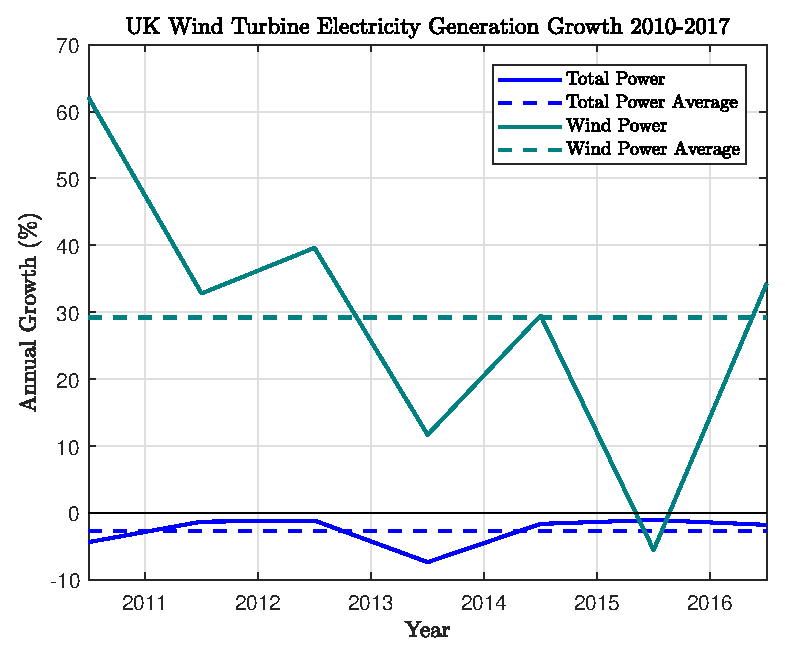
\includegraphics[width=\textwidth]{WindGrowth}
            \caption[]%
            {{\small Wind and Total Annual Growth}}    
            \label{fig:windgrowth}
        \end{subfigure}
        \caption[ The Effect of Mesh Size on Temperature Resolution ]
        {\small Statistics on UK Electrical Energy Generation} 
        \label{fig:ukenergy}
    \end{figure}

Traditionally the wind sectors growth was completely reliant on large government subsidies but in recent years governments such as the UK and Germany have adopted a new approach to subsidisation which has lead to a significant shift in the sector's economics. The policy change was to make energy companies bid for projects, and associated subsidies where available, meaning the actual subsidy received is the difference between the subsidy and the bid. This competitive approach (contract for difference) has driven innovation, with off-shore wind cost more than halving in the UK in just three years \cite{FT}. In some cases large wind projects have become viable with no subsidy or tax-break at all. The significance is the rate of development within the wind energy sector is now not reliant on government renewable energy policy but is shifting to large scale private sector investment. Due to the sheer size of the energy industry this could lead to significant wind turbine technology development. With the age of the electric car expected to dramatically reverse the trend of falling electricity consumption seen in Figure \ref{fig:ukenergy}, research into wind turbine design has never been more relevant. \\

The optimal design of a wind turbine blade is one which produces the most power for the lowest unit cost \cite{handout}. This is would require a vast amount of cost data which is not readily available and so this paper shall instead focus on the design of a technically optimal design. Specifically, the design which has the highest annual energy production (AEP) for the parameters given in Table \ref{table:parameters}. 


\begin{table}
	\centering
	\caption{Design Parameters for The Wind Turbine \cite{handout}}
	\label{table:parameters}
	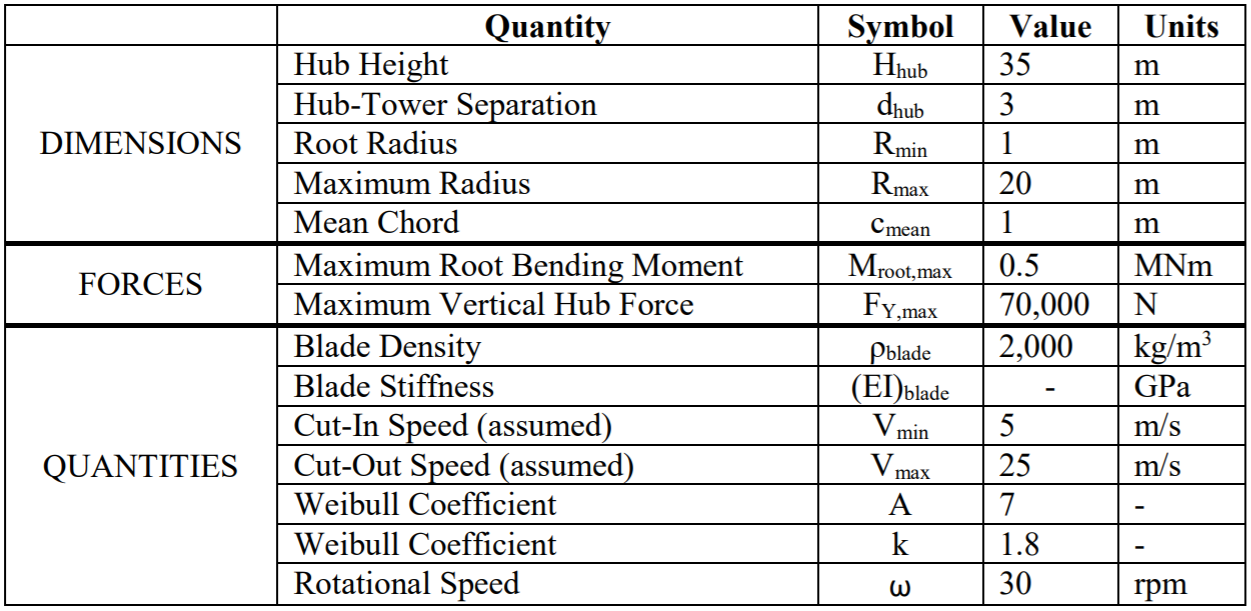
\includegraphics[width = 0.8\linewidth]{ParameterTable}
\end{table}

\FloatBarrier

%\\\\\\\\\\\\\\\\\\\\\\\\\\\\\\\\\\\\\\\\\    METHODOLOGY    \\\\\\\\\\\\\\\\\\\\\\\\\\\\\\\\\\\\\\\\\\\\\\\\\\\\\\\\\\\
\section{Methodology}

To find the optimal design blade element momentum theory was used to calculate power output for a given velocity and parameter set. Using Weibull's wind speed distribution and power output for a given velocity, AEP was calculated. Part A of the flow diagram in Figure \ref{fig:handoutflow} shows the flow of information for the computer program used to calculate the AEP.\\

\begin{figure}[h!]
\centering
	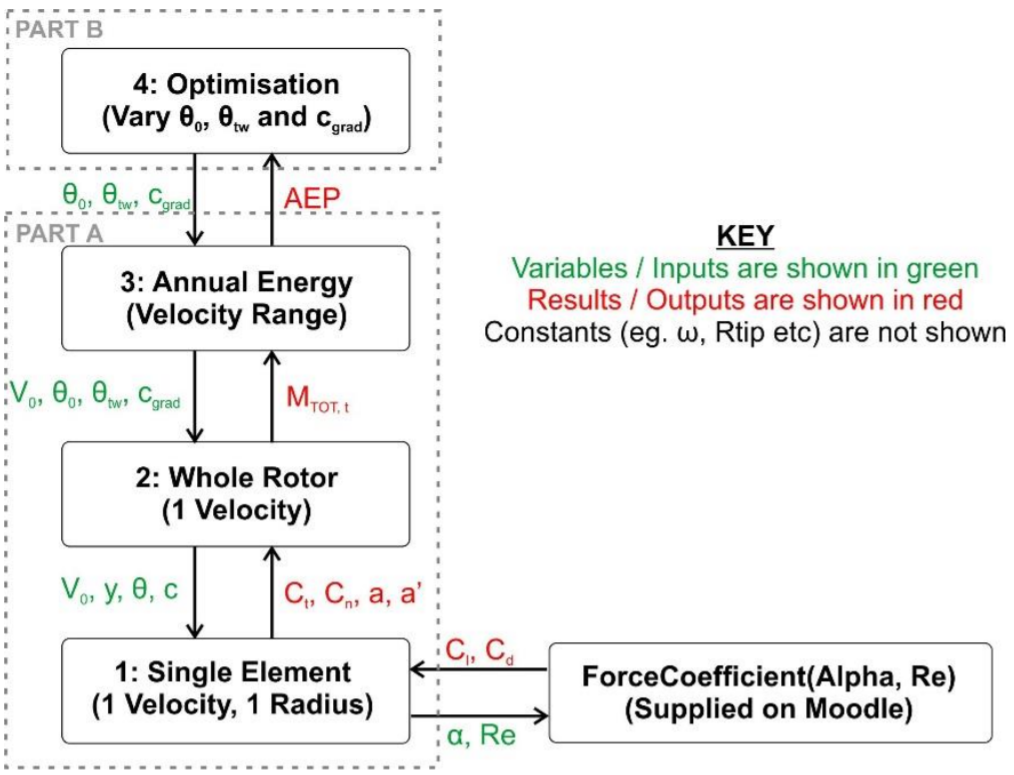
\includegraphics[width=0.75\textwidth]{HandoutFlow}
	\caption{Flow Diagram of Method Used to Find Annual Energy Production \cite{handout}}\label{fig:handoutflow}
\end{figure}

The design parameter's which could be changed for blade design were inclination at root: $\theta_0$, rate of twist: $\theta_{tw}$ and chord gradient: $c_g$. The theoretical maximum power output for a given wind speed, $V_0$, and reference area, A, is the called the Betz limit and is given by equation \ref{eq:betz}. The maximum theoretical AEP can be found using the Weibull distribution and the Betz limit. Using a minimum finding function from Matlab's library the combination of the three parameters which gives the least difference to the Betz limit AEP can be found thus finding the optimal design for the given parameter set.

\begin{equation}
	\label{eq:betz}
	P_{Betz} = \frac{16}{27} \left ( \frac{1}{2} \rho V_0^3 A \right )
\end{equation}
\FloatBarrier

%\\\\\\\\\\\\\\\\\\\\\\\\\\\\\\\\\\\\\\\\\\\\\\   RESULTS A    \\\\\\\\\\\\\\\\\\\\\\\\\\\\\\\\\\\\\\\\\\\\\\\\\\\\\\
\section{Results and Discussion}
\subsection{Part A: Calculating AEP and Initial Optimisation}
\subsubsection{Validation of Model}
The variable parameters used to interrogate the computer model are given $Set \ 1$ of Table \ref{table:setvar} . These values were first used to validate the model against known results from a correct model. This showed almost exact agreement as shown in Figure \ref{fig:validation}.

\begin{table}[!h]
\centering %Set parameters table
\ra{1.3}
\begin{tabular}{@{}ccc@{}}\toprule
 $\ Variable \ $ & $Set \ 1$ &  $Set \ 2 $\\
\midrule
$\theta_0$ & $ 12\degree$ & $ 14\degree$ \\
$\theta_{tw}$ & $ -0.4\degree/m$ \ & $ -0.3\degree/m$ \ \\
$c_{g}$ & 0 & 0\\
\bottomrule
\end{tabular}
\caption{Initial Values for Variable Parameters}
\label{table:setvar}
\end{table}


\begin{figure}
\centering
	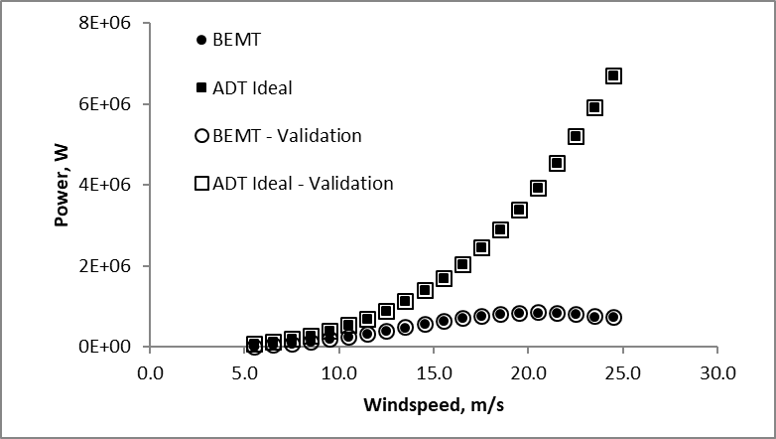
\includegraphics[width=0.75\textwidth]{validation}
	\caption{Validation of Model Against a Correct Model.}\label{fig:validation}
\end{figure}
 \FloatBarrier
\subsubsection{Power Variation with Wind Speed}
The model described by Part A  of Figure \ref{fig:handoutflow} was used to assess the effect of wind speed on power output. The result is shown by Figure \ref{fig:windspeedvpower} for the two sets of parameters given in Table \ref{table:setvar}. It can be seen that the turbine power output for $Set \ 1$ rises until approximately 22 m/s after which it begins to reduce. On the other hand the output of $Set \ 2$ increases with windspeed over the entire range and although slightly less than $Set \ 1$ until 19m/s the output for $Set \ 2$ is much greater in the 19-25 m/s region. As equation \ref{eq:betz} shows the Betz limit is proportional to velocity cubed and this behavior is evident in Figure  \ref{fig:windspeedvpower} with power output of both sets diverging from the Betz limit as wind speed increases.

\begin{figure}[ht]
\centering
	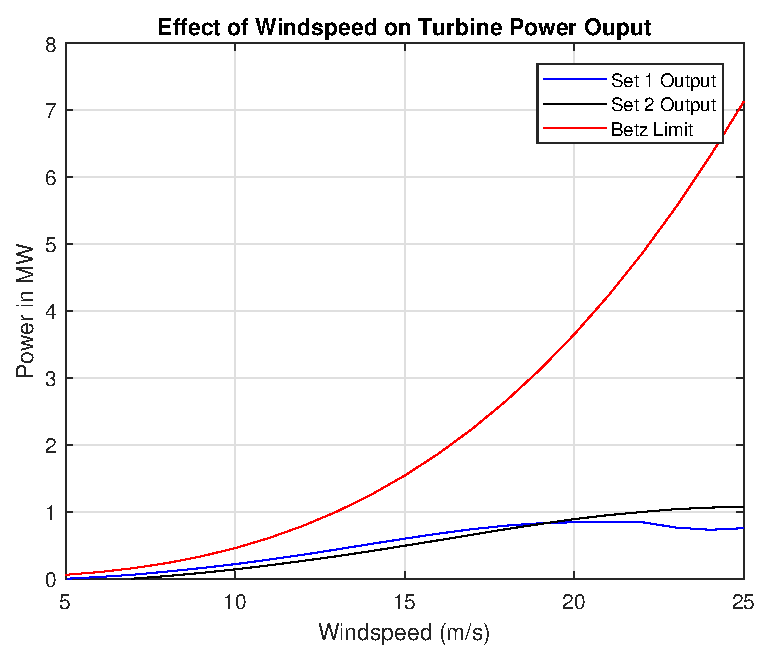
\includegraphics[width=0.75\textwidth]{WindSpeedVPower}
	\caption{Validation of Model Against a Correct Model.}\label{fig:windspeedvpower}
\end{figure}
\FloatBarrier

\subsubsection{The Weibull Distribution}

The Weibull distribution for wind speed is given by equation \ref{eq:weibull} and describes the frequency at which recorded wind speeds fall within a given speed range $V_i$ to $V_{i+1}$. The parameters k and A are unique to the geographical location and are given in Table \ref{table:parameters}. Note that this is the only equation when A does not refer to turbine reference area. The Weibull distribution over the domain 5 m/s to 25 m/s has been plotted in Figure \ref{fig:weibull}. The frequency at which windspeed exceeds 20 m/s is very low and by 25 m/s it is low enough to be insignificant which explains why cutting off generation at 25 m/s is sensible to turbine damage.


\begin{equation}
	\label{eq:weibull}
	f(V_i < V_0 < V_{i+1} ) = exp \bigg \{ - \Big( \frac{V_i}{A}\Big )^k \bigg \}  - exp \bigg \{ - \Big( \frac{V_{i+1}}{A}\Big )^k \bigg \} 
\end{equation}
\FloatBarrier
\begin{figure}[h!]
\centering
	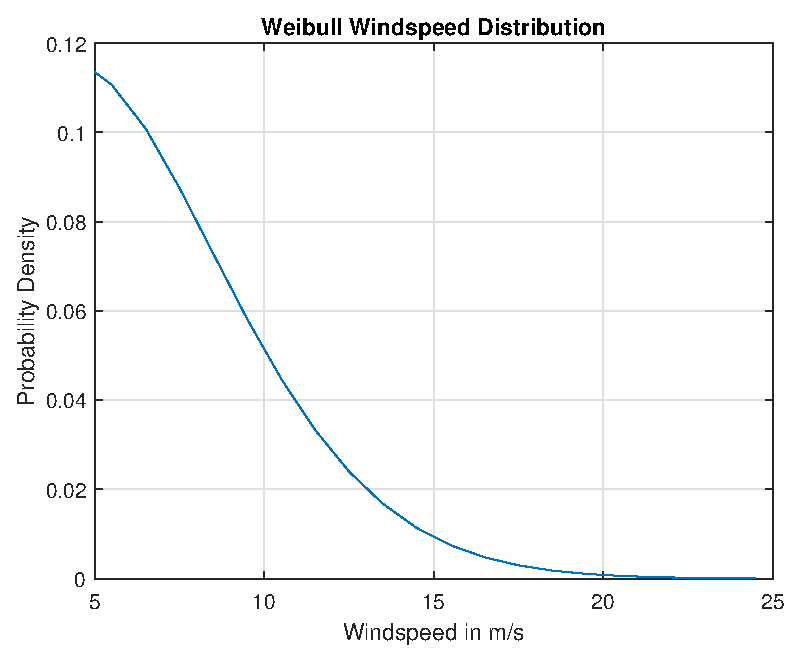
\includegraphics[width=0.75\textwidth]{Weibull}
	\caption{Weibull Windspeed Distribution with A =7 \& k = 1.8.}\label{fig:weibull}
\end{figure}

\FloatBarrier
\subsubsection{AEP: Annual Energy Production}

Figure \ref{fig:aep1} shows the power generated at each windspeed from Figure \ref{fig:windspeedvpower} multiplied by the probability density from Figure \ref{fig:weibull}. Multiplying the area under a curve by the number of hours in the year gives the AEP. It can be seen that the low frequency at which windspeeds are in excess of 20 m/s means that the amount of energy generated beyond this speed is a fraction of that produced at lower speeds. As a result the large increase in power produced by $Set \ 2 $ turbine compared to $Set \ 1$ at speeds at over 20 m/s is indistinguishable from Figure \ref{fig:aep1}. Contrastingly the  small increase in power generation of $Set \ 1$ over the 5 m/s to 20m/s speed range has been amplified by the high wind frequency in this region making it a much more effective design.

\begin{figure}[h!]
\centering
	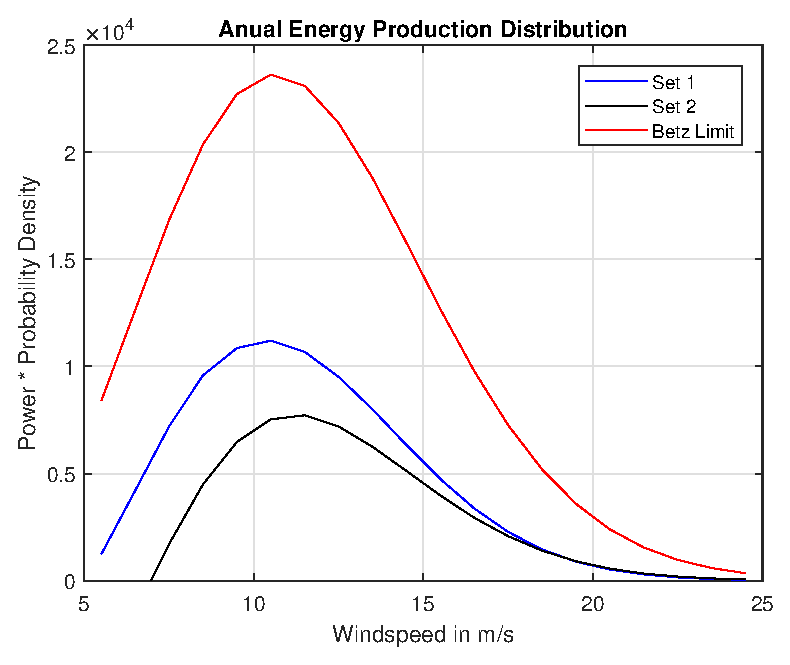
\includegraphics[width=0.75\textwidth]{AEP1}
	\caption{Power Multiplied by Probability Density for Each Windspeed}\label{fig:aep1}
\end{figure}


\begin{table}[!h]
\centering %Set parameters table
\ra{1.3}
\begin{tabular}{@{}lcccl@{}}\toprule
 $\ Variable \ $ & Betz & Set 1 &  Set 2 & Units \\
\midrule
AEP \   & 2000 &$ 811 $ & $ 463 $ & $(MWhr/year)$ \\
$\%$ \ of  \ Betz & - &$ 41 $\ & $ 23$  & $ \%$\ \\
\bottomrule
\end{tabular}
\caption{Initial Values for Variable Parameters}
\label{table:setcomp}
\end{table}


\subsubsection{Optimal Design}

The optimal design is the design for which the AEP is the highest percentage of the Betz limit AEP. The first stage in finding this set of parameters was to investigate the effect of each parameter individually. Using the parameters of Set 1 each parameter was adjusted with the rest remaining as the values from Set 1. Figures \ref{fig:changetheta01} and \ref{fig:changetwist} show the effect of changing $\theta_0$ and $\theta_{tw}$ on AEP respectively. Reading off the peaks approximately gives the optimal values of $ \theta_0 = 7.5 \degree$ and $\theta_{TW} = -0.7 \degree/m$. 

\begin{figure}[ht] 
        \centering
        \begin{subfigure}[b]{0.475\textwidth}
            \centering
            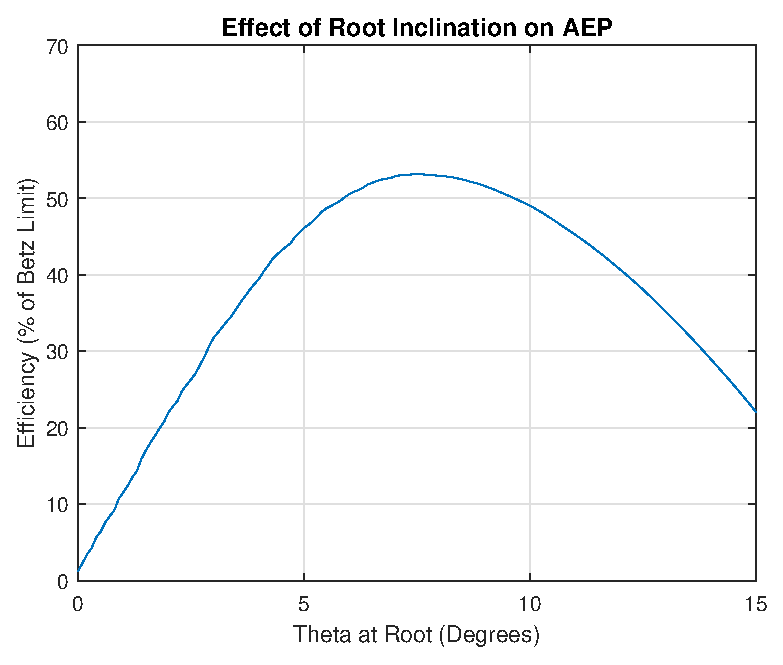
\includegraphics[width=\textwidth]{ChangeTheta0}
            \caption[Network2]%
            {{\small The Effect of Root Inclination. }}    
            \label{fig:changetheta01}
        \end{subfigure}
        \hfill
        \begin{subfigure}[b]{0.475\textwidth}  
            \centering 
            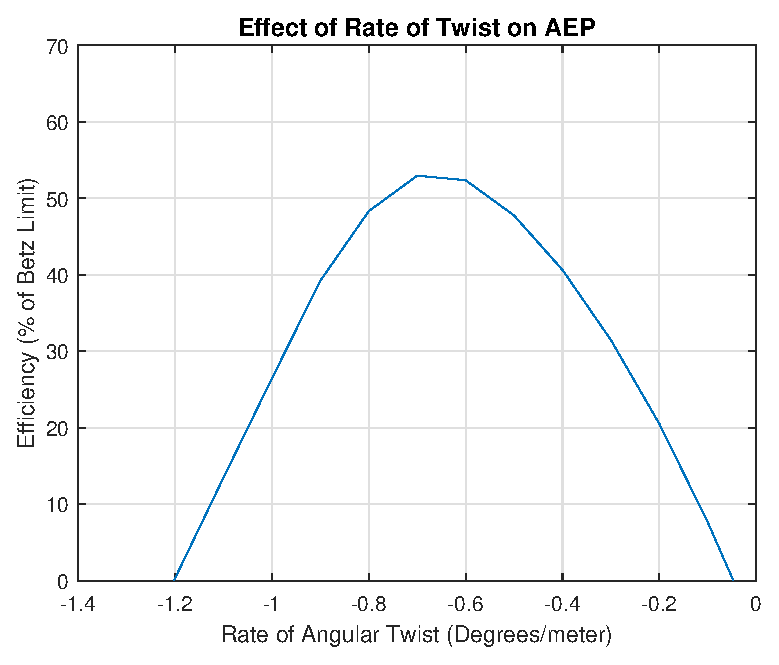
\includegraphics[width=\textwidth]{ChangeThetaTW.eps}
            \caption[]%
            {{\small The Effect of Rate of Twist. }}    
            \label{fig:changetwist}
        \end{subfigure}
        \caption{Effect of Angular Parameters on Turbine AEP.}
        \label{fig:changetheta}
    \end{figure}
\FloatBarrier
The effect of chord gradient was also investigated and the result is shown in Figure \ref{fig:changegrad}. The Figure shows AEP increases with increasing chord gradient. Larger chords give greater lift and so with the highest chord gradient there will be the greatest lift at the tip of the blade. This can be explained as rotational power is proportional to force, radius and rotational velocity. With rotational velocity set at 30rpm, by having lift increase with radius the maximum power output will be obtained. In reality turbine blades are not designed with large positive chord gradients and the model was later improved to reflect this. Temporarily disregarding this the chord gradient is only limited by the requirement to have a positive chord at 20m radius and at least 0.4m chord at the root for attaching to hub.\\

\begin{figure}[h!]
\centering
	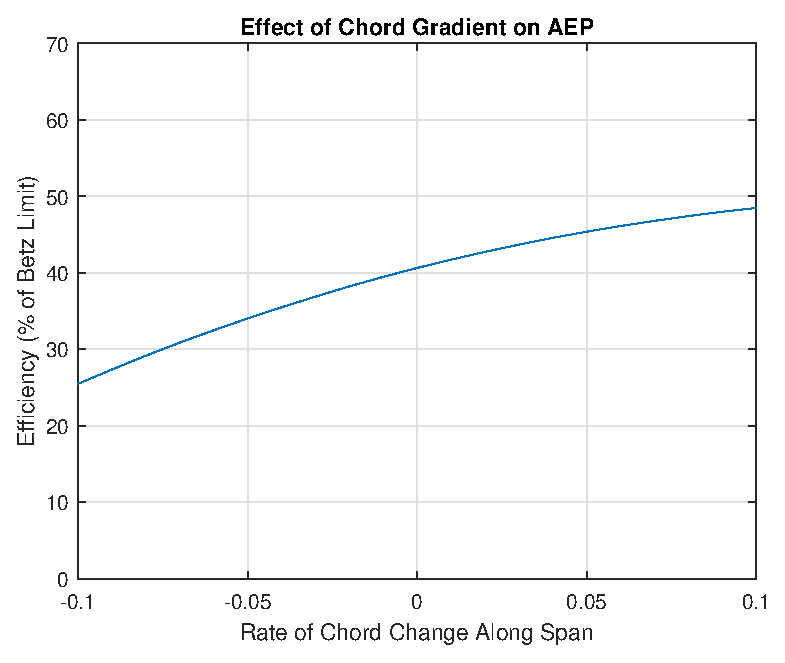
\includegraphics[width=0.475\textwidth]{ChangeGrad}
	\caption{Effect of Chord Gradient on Turbine AEP.}\label{fig:changegrad}
\end{figure}
\FloatBarrier
A cost function was created which outputted the difference between AEP and the Betz limit AEP. A minimum finding algorithm was then used to find the values of $\theta_0$, $\theta_{TW}$ and $c_g$ which gave the optimum AEP. The result is shown in Table \ref{table:simpleresult}. 


\begin{table}[!h]
\centering %Set parameters table
\ra{1.3}
\begin{tabular}{@{}lcl@{}}\toprule
\ \textbf{Parameter}  & \textbf{Value}  &  \textbf{Units} \\
\midrule
$\theta_0$  & 7.9 & $\degree$ \ \\
$\theta_{TW}$ & -0.37 & $\degree/m$  \\
$c_{g}$ & 0.084 & m/m \ \\
\midrule
AEP  & 1,190 & MWhr/year\ \\
\% of Betz & 59.8 & \% \ \\
\midrule
$M_{root,max}$ & 0.6 & MNm \\
Tip Deflection  & $>3$ & m \\
\bottomrule
\end{tabular}
\caption{Optimum for Initial Model}
\label{table:simpleresult}
\end{table}

The function has improved efficiency compared to $\text{AEP}_{Betz}$ to 59.8\% compared to 41\% for the Set 1 starting case. The values are similar to those predicted from initial analysis which gives confidence that the minimum finding function has worked correctly. The criteria for tip deflection  (maximum 3m) and maximum root bending moment (0.5MNm) were not met however and so this design is not viable. The chord gradient tended to the maximum which was constrained at 0.084 and the resulting high loads at the tip of the blade caused the excessive bending moment and deflection. Therefore an improved model was needed to keep these parameters below the requirements.


\FloatBarrier
\subsection{Part B: Limitations of Model and Enhancements}

\subsubsection{Limitations of Model}
The model used in section A had several limitations which could be categorised into geometric, aerodynamic and structural. \\

\begin{itemize}
\item{\textbf{Geometric:}}
\begin{enumerate}
\item{\textit{Linear Taper} - This is a fair simplification overall but near the tip, where velocities are large, a more complex shape or second taper rate may be optimal.}
\item{\textit{Linear Twist} - This simplifies the optimisation process but a non linear twist would likely increase AEP.}
\end{enumerate}
\item{\textbf{Aerodynamic:}}
\begin{enumerate}
\item{\textit{Tip Losses} - These have not been modelled which may have contributed to the unrealistic chord gradient (or taper rate) result.}
\item{\textit{Compressibilty} - No check for compressible flow at tip but as low speed operation this is reasonable assumption.}
\item{\textit{Noise} - An technically optimal design should have noise limits. Large tip chords produce lots of noise so this aspect design should be considered.}
\item{\textit{Small Values of a} - Assumed that $a$ will not exceed 0.4 and so the Glauert Correction for a is not needed \cite{Hansen}.}
\end{enumerate}
\item{\textbf{Structural:}}
\begin{enumerate}
\item{\textit{Fatigue} - Fatigue considerations would give life of blade and optimisation could therefore be attempted for life of blade rather than single year. A blade which has 10\% lower AEP is a much better design if it has 25 \% longer life for example.}
\item{\textit{Root Bending Moment} - This needs to be added to model to check it does not exceed the maximum specified in Table \ref{table:parameters}. }
\item{\textit{Tip Deflection} - If tip deflection exceeds 3m the tip will collide with the tower and so the model needs to ensure this does not happen.}
\end{enumerate}
\end{itemize}


\subsubsection{Adding Bending Analysis to Model}
The most important limitations to correct were the root bending moment and tip deflection as then it could be assured the conditions in Table \ref{table:parameters} are met. A new function was created to calculate these design parameters using a modified version of the method described by Hansen \cite{Hansen}. The beam is discretized as shown in Figure \ref{fig:discretebeam}. Using the existing model the normal moments were found at each node as described by equation \ref{eq:momentnormal}. 

\begin{figure}[h!]
	\centering
	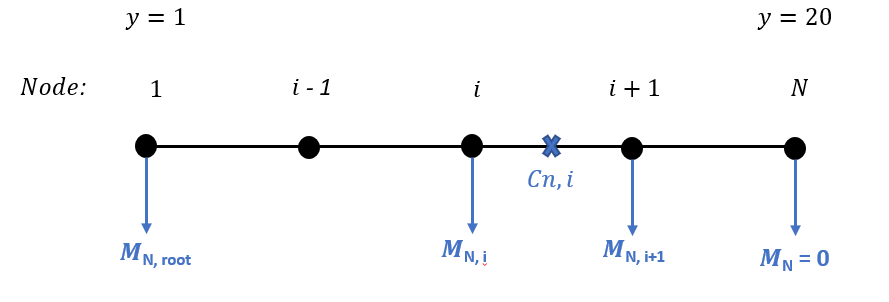
\includegraphics[width=0.75\textwidth]{DiscreteBeam}
	\caption{Discrete Beam for Deflection Analysis.}\label{fig:discretebeam}
\end{figure}

\begin{equation}
	\label{eq:momentnormal}
	M_{N,i} = M_{N,i} + c_{N,i+1}*(0.5\rho V_{rel}^2)*(y_{i+1}-y_{i})*y_{i}
\end{equation}
\FloatBarrier

The tangential bending moment was calculated in the same way after which the root bending moment was calculated using equation \ref{eq:momentroot} with $V_0 = 25 m/s$.

\begin{equation}
	\label{eq:momentroot}
	M_{root} = (M_{N,1} + M_{N,1})^{0.5}
\end{equation}
\FloatBarrier

The AEP was set to zero if the tip deflection or root bending moment exceeded the limits from Table \ref{table:parameters}. This led to a new optimum design which is displayed in Table \ref{table:bendingresults} along with the initial model values for comparison. It should be noted that centrifugal force will resist motion and to improve accuracy the effect should have been accounted for.

\begin{table}[!h]
\centering %Set parameters table
\ra{1.3}
\begin{tabular}{@{}lccl@{}}\toprule
\ \textbf{Parameter}  & \textbf{Initial Model}  & \textbf{Bending Model} &  \textbf{Units} \\
\midrule
$\theta_0$  & 7.9 & 11 & $\degree$ \ \\
$\theta_{TW}$ & -0.37 & -0.6 & $\degree/m$  \\
$c_{g}$ & 0.084 & .006 & m/m \ \\
\midrule
AEP  & 1,190 & 1,080 & MWhr/year\ \\
\% of Betz & 59.8 & 54.2 & \% \ \\
\midrule
$M_{root,max}$ & 0.6 & 0.46 & MNm \\
Tip Deflection  & $>>3$ & 3.0 & m \\
\bottomrule
\end{tabular}
\caption{Comparison Between Initial and Bending Models}
\label{table:bendingresults}
\end{table}

As expected the chord gradient was much reduced after implementing bending restriction now almost straight  at $c_g = 0.006$. The restrictions also reduced the AEP of output to \mbox{54.2\%}  from \mbox{59.8\%} of the Betz limit. \\

\subsubsection{Adding Tip Losses to Model}

As the optimal solution was had a slightly positive chord gradient the effect of tip losses was deemed potentially significant. Prandtl's tip loss correction factor was applied to the model in addition to the bending checks. The result has been added to Table \ref{table:bendingresults} to produce Table \ref{table:finalresults}. 

\begin{table}[!h]
\centering %Set parameters table
\ra{1.3}
\begin{tabular}{@{}lcccl@{}}\toprule
\ \textbf{Parameter}  & \textbf{Initial Model}  & \textbf{+ Bending } & \textbf{+ Tip Losses} & \textbf{Units} \\
\midrule
$\theta_0$  & 7.9 & 11 & 9.87 & $\degree$ \ \\
$\theta_{TW}$ & -0.37 & -0.6 & -0.54 & $\degree/m$  \\
$c_{g}$ & 0.084 & .006 & .008 & m/m \ \\
\midrule
AEP  & 1,190 & 1,080 & 991 & MWhr/year\ \\
\% of Betz & 59.8 & 54.2 & 49.7 & \% \ \\
\midrule
$M_{root,max}$ & 0.59 & 0.46 & 0.44 & MNm \\
Tip Deflection  & $>>3$ & 3.0 & 3.0 & m \\
\bottomrule
\end{tabular}
\caption{Comparison Between Initial, Initial with Bending and Initial with Bending and Tip Losses Models}
\label{table:finalresults}
\end{table}

The tip loss addition was significant and led to a 8.2 \% reduction in AEP. The comparison with the Betz limit can be seen graphically in Figure \ref{fig:finalcomp}. For the final parameters the values of $a$ very rarely exceeded 0.4 and so, although not ideal, the abscence of Glauert's correction factor is deemed acceptable.

\begin{figure}[h!]
	\centering
	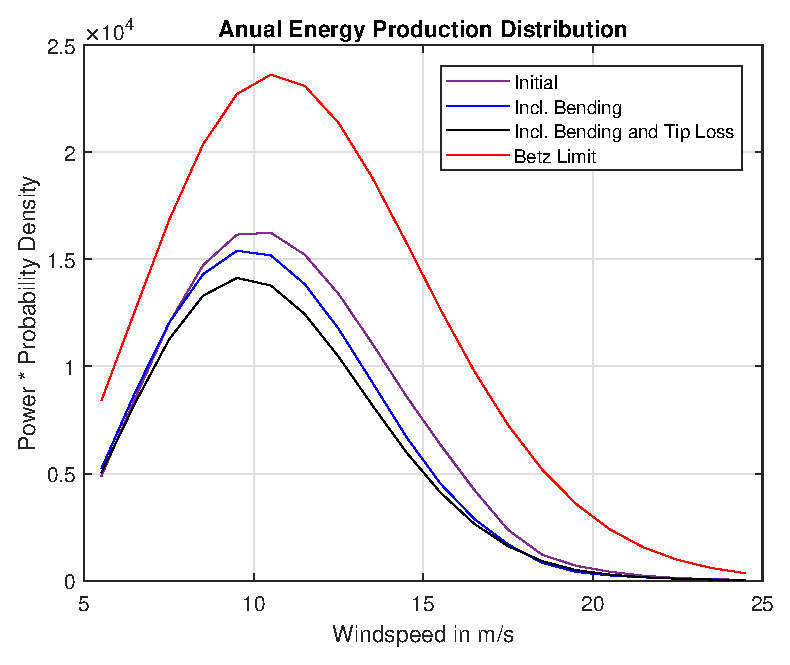
\includegraphics[width=0.75\textwidth]{AEPFinal}
	\caption{Comparison AEP as Features Were Added to Model.}\label{fig:finalcomp}
\end{figure}

\subsubsection{Final Design}

The final design chosen was the optimal design which included tip losses and bending analysis. Using the  parameters from Table \ref{table:finalresults} and the set parameters from Table \ref{table:parameters} a CAD model of the blade was made. The aerofoil used for the CAD model was a NACA 0012 as this is where the force coefficient data was derived from. The resulting engineering drawing is shown in Figure \ref{fig:CAD}. It should be noted that the values of $\theta_0$ from Table \ref{table:finalresults} are at $y = 0m$, so the at the root, where $y = 1m$, the actual inclination is: $\theta_{ROOT} = \theta_0 + \theta_{TW}$\\
The CAD model was also used to calculate the weight of the blade and it was found that the `Maximum Vertical Hub Force' was exceeded by the weight of the three blades.

\begin{table}[!h]
\centering %Set parameters table
\ra{1.3}
\begin{tabular}{@{}lcl@{}}\toprule
 $\ Variable \ $ & Value &  $Units $\\
\midrule
Blade Density &  2000 & $ kg/m^3$ \\
Blade Volume& 1.57 \ & $ m^3$ \ \\
Single Blade Mass & 3,150 \ & $ kg$ \ \\
Number of Blades & 3 & \\
\midrule
Maximum Vertical Hub Force & 70,000 & $N$ \\
Combined Weight of Blades &  92,600 & $N$ \\
\bottomrule
\end{tabular}
\caption{Weight Data for Final Design}
\label{table:weight}
\end{table}


\begin{figure}[p]  %nrcVrc Figure
	\centering
	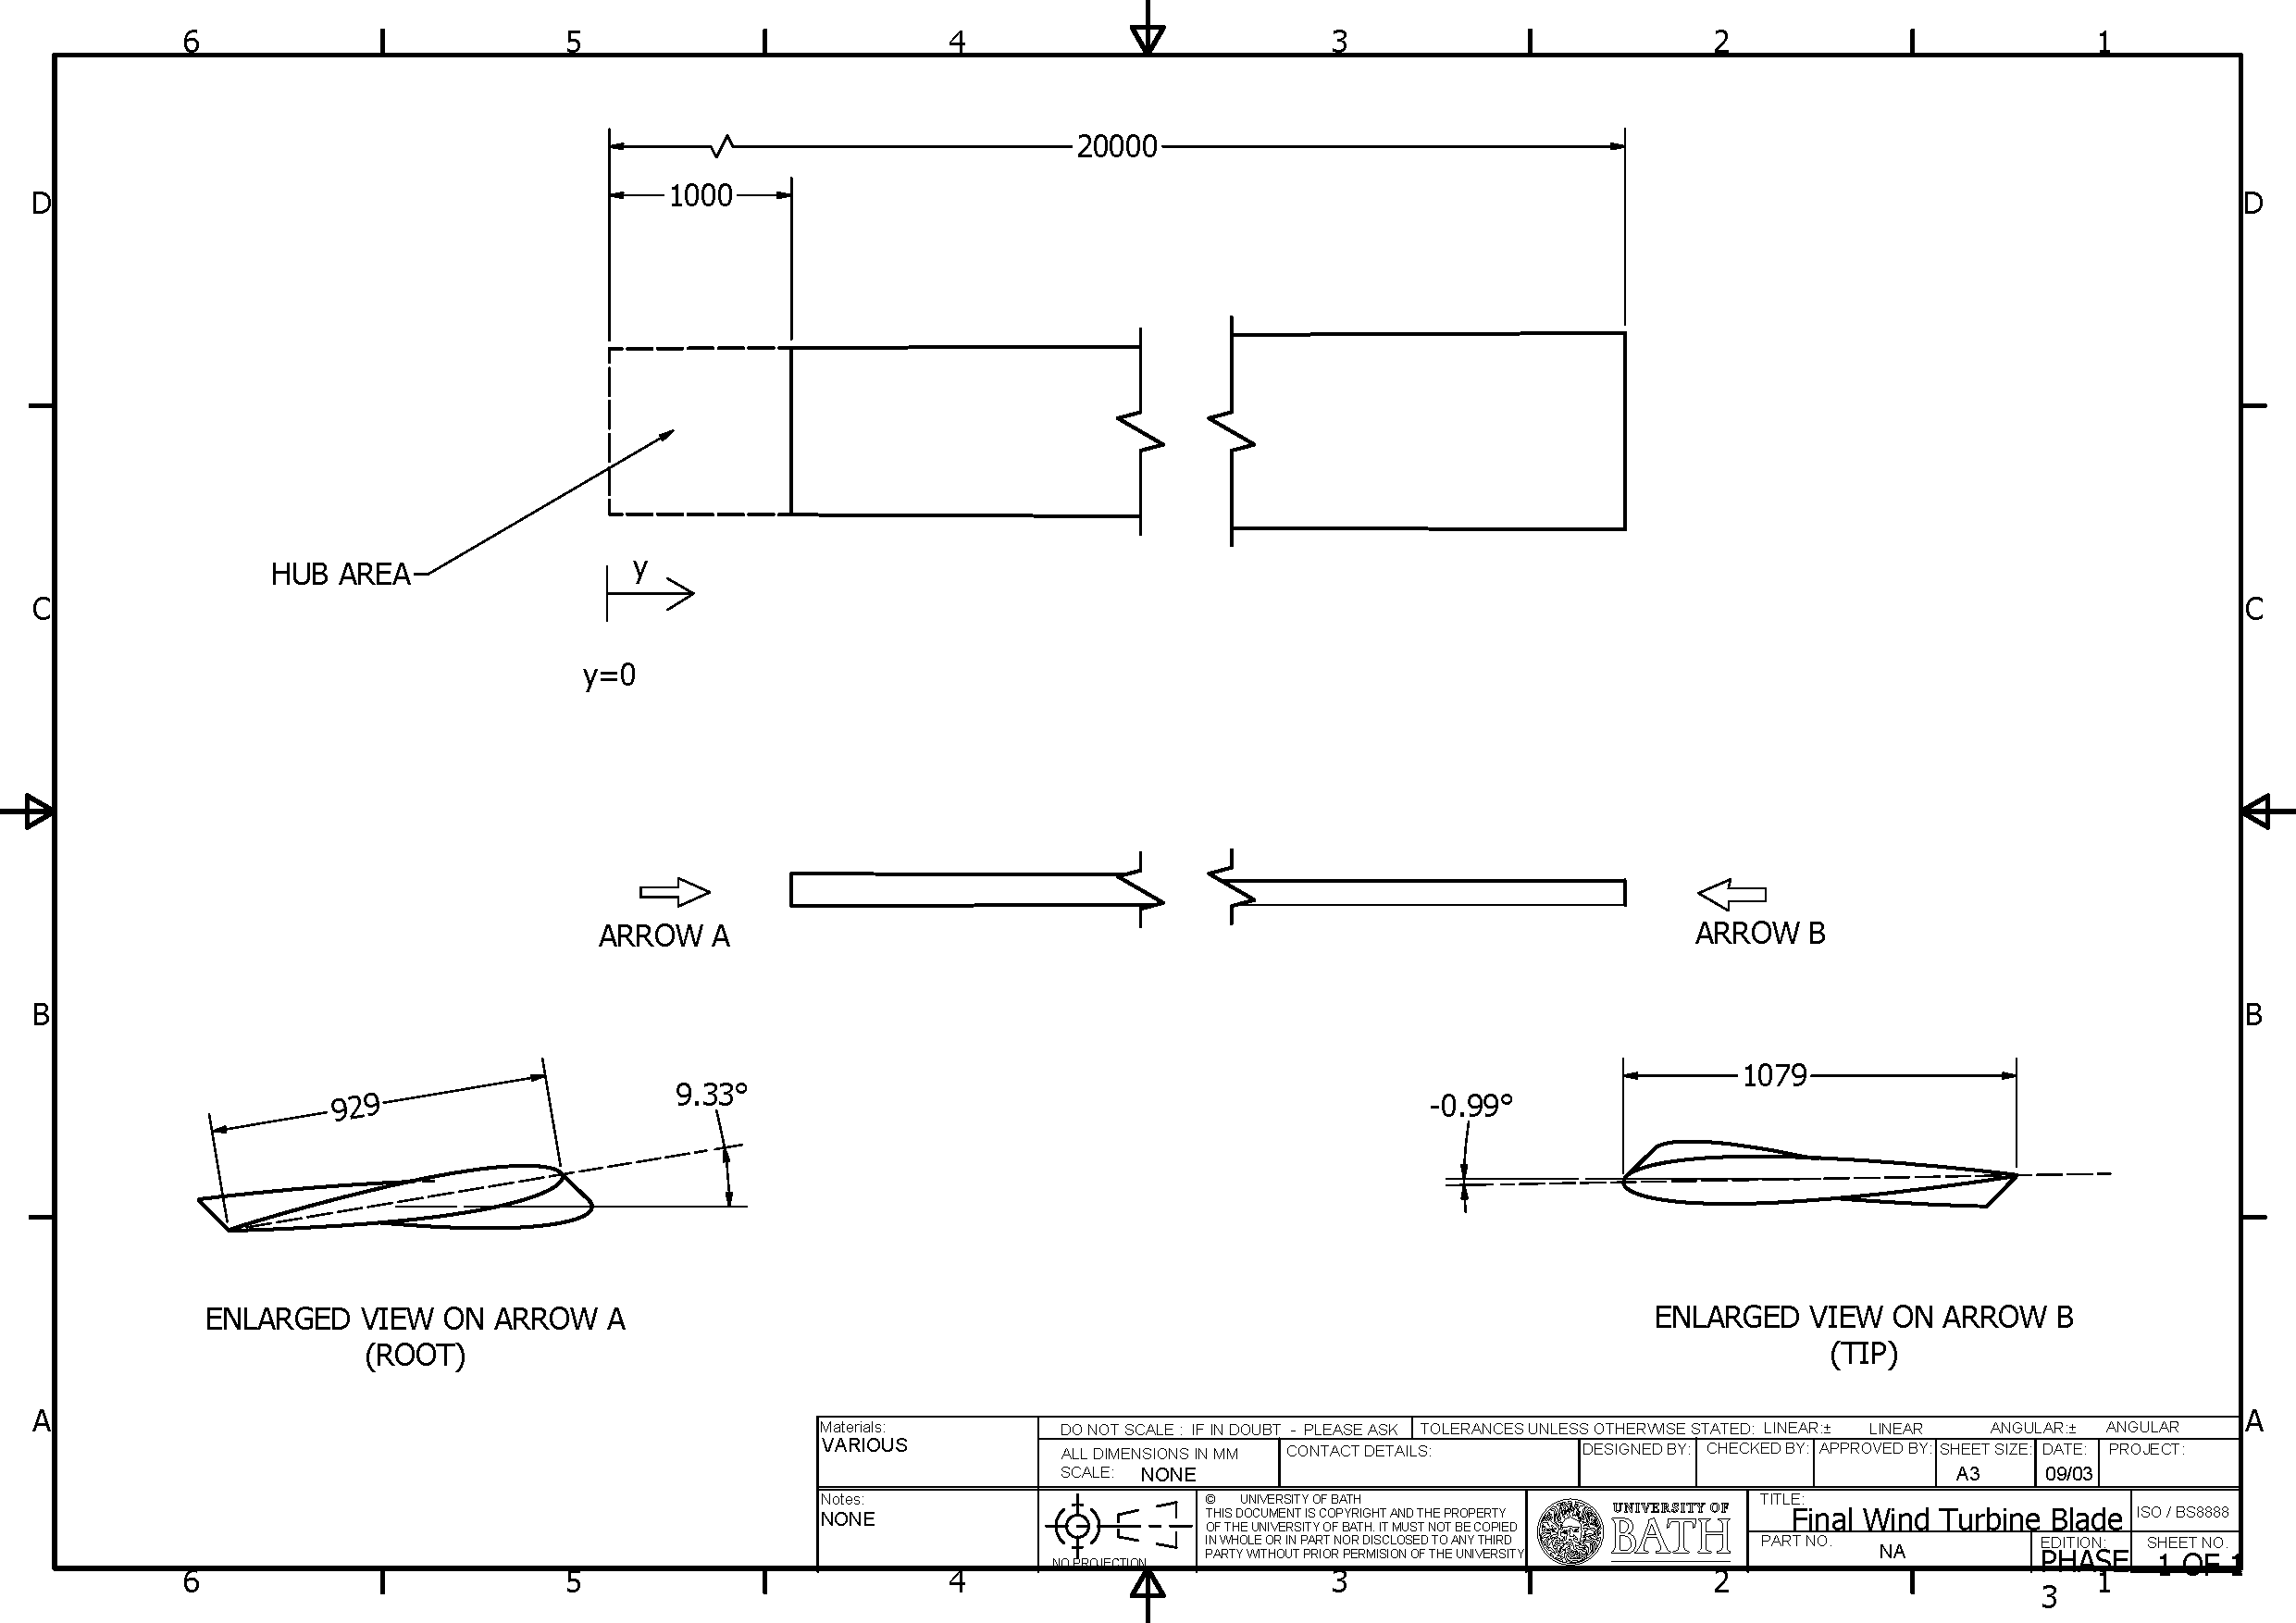
\includegraphics[width=1.2\textwidth, angle=270]{WTBlade}
	\caption{Drawing of Final Design.}
	\label{fig:CAD}
\end{figure} 

\FloatBarrier
\section{Conclusions}

A first stage design was found which had an AEP which was 49.7\% of the Betz limit. All criteria were met except weight restrictions and so a lighter construction material would be required. Some major assumptions in the original model were accounted for to obtain a realistic design, with tip deflection becoming a limiting factor for chord gradient and tip losses reducing maximum AEP by 8.2 \%. Despite many further limitations of the model due to the simple linear twist and taper design input parameters the model was indeed suitable. To improve the design it is suggested to implement additional linear twist rate or a non-linear twist and have a bespoke designed tip. With the more advanced design some more of the limitations discussed in the report should be accounted for.







\begin{thebibliography}{9}
%Last name, First Initial, Year published. Title. Publisher, Volume, Page(s).
% HARVARD REFERENCE STYLE:
%Brunner, F.H., 1949. Synthetic gasoline from natural gas. Industrial and engineering chemistry, 41(11), pp.2511-2515.

\bibitem{data1} 
Department for Business, Energy \& Industrial Stratergy, 2018. 
\textit{Historical Electricity Data:1920 to 2017.}\\
Available: www.gov.uk/government/statistical-data-sets/historical-electricity-data

\bibitem{data2} 
Digest of United Kingdom Energy Statistics (DUKES), 2018. 
\textit{Digest of UK Energy Statistics (DUKES): electricity.}
Available:https://www.gov.uk/government/collections/electricity-statistics

\bibitem{moodleslides} 
Cleaver, D., 2018. 
\textit{Slides: WT Coursework.}\\
University of Bath.

\bibitem{handout} 
Cleaver, D., 2018. 
\textit{ME40343 Helicopter Dynamics: Coursework.}\\
University of Bath.

\bibitem{guardian} 
Vaughan, A., 2017. 
\textit{Electric cars will fuel huge demand for power, says National Grid.}\\
The Guardian.

\bibitem{FT}
Arie, S., 2018. 
\textit{Renewables are primed to enter the global energy race.}\\
The Financial Times.

\bibitem{Hansen}
Hansen, M.O.L., 2000. 
\textit{Aerodynamics of Wind Turbines.}\\

\end{thebibliography}


\pagebreak

\begin{appendices}

%%AAAAAAAAAAAAAAAAAAAAAAAAAA%%%%%%%
\section{Induced Calculations Function}\label{ap:induced}

\lstinputlisting[style=Matlab-editor]{C:/Users/xav_m/OneDrive/Documents/XAVI/University/Final_Year/HELICOPTERS/Coursework/Windturbine_Optimisation/WTInducedCalcs.m}

\section{Wind Turbine Single Velocity Function}\label{ap:single}
\lstinputlisting[style=Matlab-editor]{C:/Users/xav_m/OneDrive/Documents/XAVI/University/Final_Year/HELICOPTERS/Coursework/Windturbine_Optimisation/WTSingleVelocity.m}

\section{Wind Turbine Velocity Range Function}\label{ap:range}
\lstinputlisting[style=Matlab-editor]{C:/Users/xav_m/OneDrive/Documents/XAVI/University/Final_Year/HELICOPTERS/Coursework/Windturbine_Optimisation/WTVelocityRange.m}

\section{Wind Turbine Velocity Range Function}\label{ap:optimisation}
\lstinputlisting[style=Matlab-editor]{C:/Users/xav_m/OneDrive/Documents/XAVI/University/Final_Year/HELICOPTERS/Coursework/Windturbine_Optimisation/TurbineOptimisation.m}

\section{Flow Chart of FEM Solver}
%\begin{lstlisting}
%function [SqMatrix] = LaplaceElemMatrix(D, eID, msh)
%
%%Returns the local 2x2 element matrix of a given element for a given diffusion
%%coefficient
%%
%% Inputs: 
%% D - Coefficient of Diffusion
%% eID - Index of element within mesh structure
%% msh - Mesh which contains local elements within it's structure
%
%%% Form of Laplace Elem matrix for J=1, D=1
%
%SqMatrix = [0.5, -0.5; ...
%            -0.5, 0.5];
%
%%% Multiply  by (1/J) and D to get solution for the particular element
%
%J = msh.elem(eID).J;  %Get Jacobi for the element
%
%SqMatrix = (1/J) * D * SqMatrix;   %Local element matrix for element eID
%end
%\end{lstlisting}
%\pagebreak










\end{appendices}





\end{document}

